\Cref{fig:overview} gives a graphical overview of the data flow between the components involved in the architectural changes of this document.
To keep the diagram simple, not all dependencies are indicated; for example, many components require access to a recent ledger state in order to validate votes or certificates or to decide whether to cast a vote.
We elide all existing components that do we do not expect to modify non-trivially.

\begin{figure}[h]
  \centering

  \usetikzlibrary{arrows.meta, fit}
  \pgfdeclarelayer{background}
  \pgfsetlayers{background, main}

  \begin{adjustbox}{scale=0.75}
  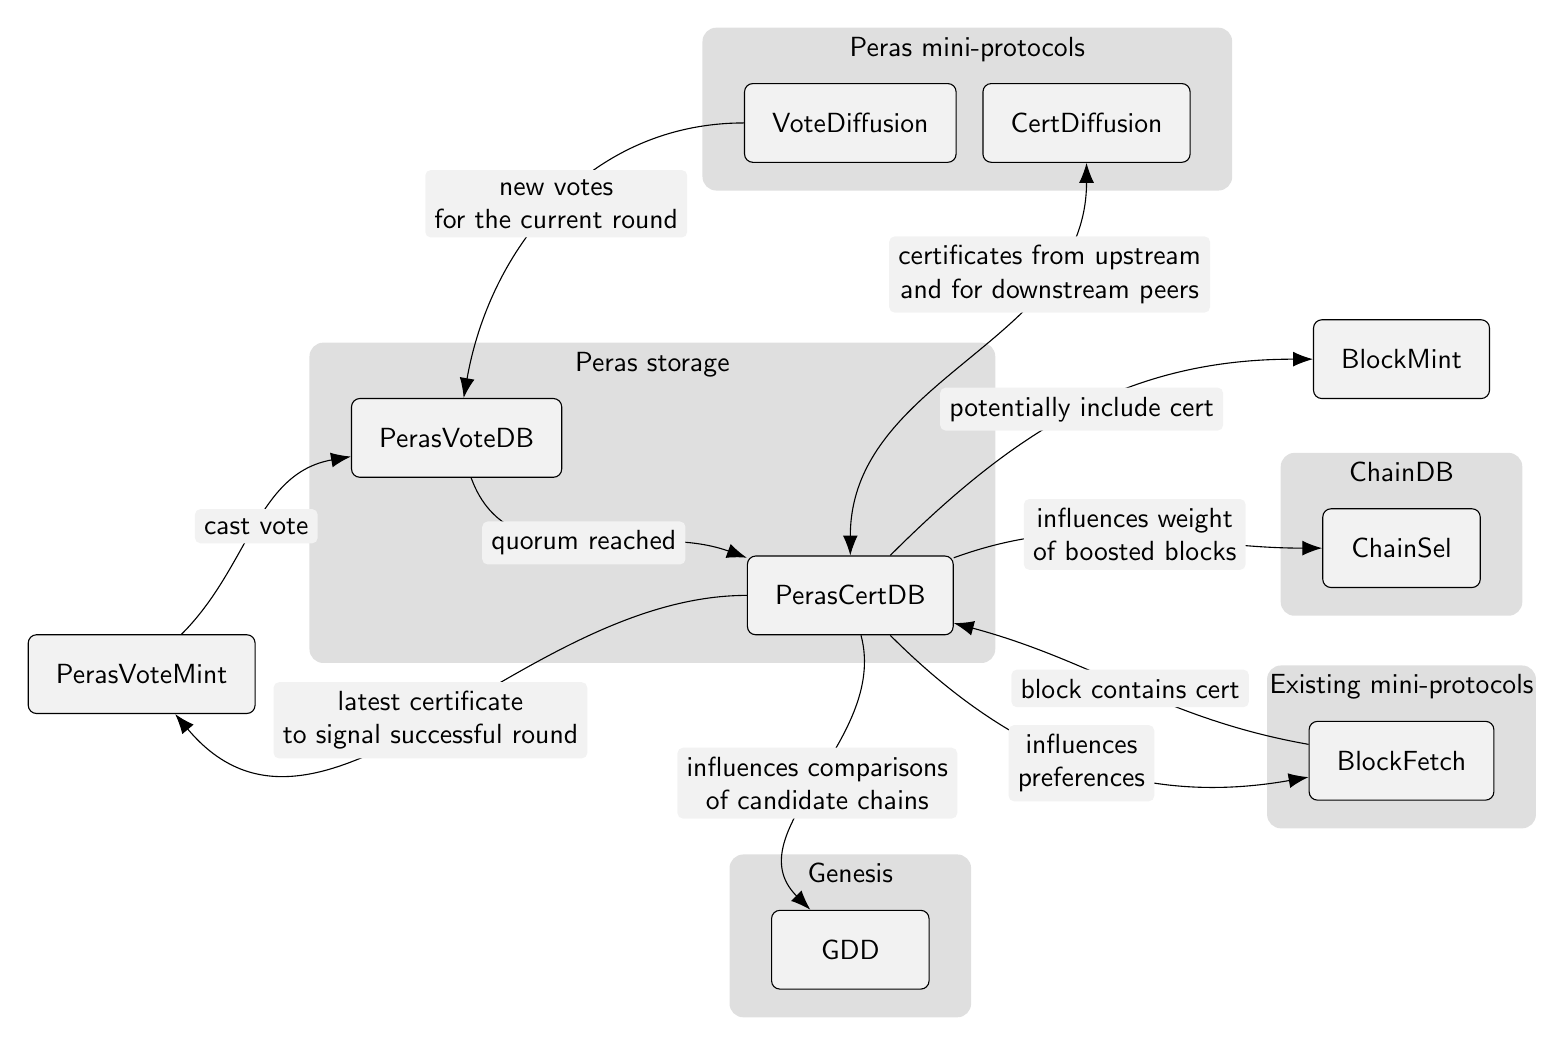
\begin{tikzpicture}[
      every node/.style={
        font=\sffamily,
        text=black,
      },
      component/.style={
        draw,
        fill=gray!10,
        rounded corners=3pt,
        minimum width=2cm,
        minimum height=1cm,
        align=center,
        inner xsep=10pt,
        inner ysep=2pt,
      },
      label/.style={
        fill=gray!10,
        rounded corners=2pt,
      },
      grouping/.style={
        rounded corners=5pt,
        inner xsep=15pt,
        inner ysep=15pt,
        yshift=5pt,
        fill=gray!25,
      },
      >={Latex[scale=1.5]},
    ]

    \node[component] (PerasVoteMint) at (0, -3) {PerasVoteMint};
    \node[component] (PerasVoteDB) at (4, 0) {PerasVoteDB};
    \node[component] (PerasCertDB) at (9, -2) {PerasCertDB};

    \node[component] (VoteDiffusion) at (9, 4) {VoteDiffusion};
    \node[component] (CertDiffusion) at (12, 4) {CertDiffusion};
    \node[component] (BlockMint) at (16, 1) {BlockMint};
    \node[component] (ChainSel) at (16, -1.4) {ChainSel};
    \node[component] (BlockFetch) at (16, -4.1) {BlockFetch};
    \node[component] (GDD) at (9, -6.5) {GDD};

    \draw[->, out=45, in=-170] (PerasVoteMint) to node[label, midway]{cast vote} (PerasVoteDB);
    \draw[->, out=-70, in=160] (PerasVoteDB) to node[label, midway]{quorum reached} (PerasCertDB);
    \draw[<-, out=80, in=180] (PerasVoteDB) to node[label, midway,align=center]{new votes\\for the current round} (VoteDiffusion) {};
    \draw[<->, out=90, in=270] (PerasCertDB) to node[label, near end,align=center]{certificates from upstream\\and for downstream peers} (CertDiffusion);
    \draw[->, out=45, in=180] (PerasCertDB) to node[label, midway]{potentially include cert} (BlockMint);
    \draw[->, out=20, in=180] (PerasCertDB) to node[label, midway, align=center]{influences weight\\of boosted blocks} (ChainSel);
    \draw[<-, out=-15, in=170] (PerasCertDB) to node[label, midway]{block contains cert} (BlockFetch);
    \draw[->, out=-45, in=190] (PerasCertDB) to node[label, midway, align=center]{influences\\preferences} (BlockFetch);
    \draw[->, out=-75, in=135] (PerasCertDB) to node[label, midway, align=center]{influences comparisons\\of candidate chains} (GDD);
    \draw[->, out=180, in=-50] (PerasCertDB) to node[label, midway, align=center]{latest certificate\\to signal successful round} (PerasVoteMint);

    \begin{pgfonlayer}{background}
      \node[grouping, fit={(PerasVoteDB) (PerasCertDB)}] (Peras storage) {};
      \node[anchor=north, overlay] at (Peras storage.north) {Peras storage};

      \node[grouping, fit={(VoteDiffusion) (CertDiffusion)}] (Peras mini-protocols) {};
      \node[anchor=north, overlay] at (Peras mini-protocols.north) {Peras mini-protocols};

      \node[grouping, fit={(ChainSel)}] (ChainDB) {};
      \node[anchor=north, overlay] at (ChainDB.north) {ChainDB};

      \node[grouping, fit={(BlockFetch)}] (Existing mini-protocols) {};
      \node[anchor=north, overlay] at (Existing mini-protocols.north) {Existing mini-protocols};

      \node[grouping, fit={(GDD)}] (Genesis) {};
      \node[anchor=north, overlay] at (Genesis.north) {Genesis};
    \end{pgfonlayer}

    %% \begin{pgfonlayer}{background}
    %%   \draw[dashed, rounded corners=.3cm, fill=lightgray]
    %%   (right-of-shell)
    %%   |- (above-colis)
    %%   -| (left-of-specs)
    %%   |- (below-exec)
    %%   -| node[midway,above left]{colis-language}
    %%   (right-of-ast)
    %%   |- (above-cst)
    %%   -| cycle;
    %% \end{pgfonlayer}
  \end{tikzpicture}
  \end{adjustbox}

  \caption{Overview of the data flow between the components of this document}%
  \label{fig:overview}
\end{figure}


%%% Local Variables:
%%% mode: latex
%%% TeX-engine: xetex
%%% TeX-master: "../peras-design"
%%% End:
